\section{Results}
The results section is divided into three subsections, each corresponding to the individual research questions as described in the \textit{introduction} section. (R1) Relates to the activity of political parties on the platform, (R2) relates to topics from election manifestos and voting guides, and (R3) relates to network analysis of instances and servers of political parties on the network. Each with accompanying descriptions of the methods performed and graphs to further understand the data and the result of the analysis.

A clear increase in general activity surrounding the Dutch elections on the platform is found.
When querying toots with general terms on Dutch elections, for example, “verkiezingen”, “dutch elections”, or “tweede kamer”, the results have very clearly spiked in the last period, as shown in figure \ref{fig:electionstotal}. A total of 18,230 toots were retrieved, which included these election-related terms, of which around 16,000 were in the last two years.
Therefore, Mastodon has been more widely adopted for the most recent election year, 2023, as opposed to previous elections, 2017 and 2021, which showed almost no activity on these general queries.

\begin{figure}[ht]
  \centering
  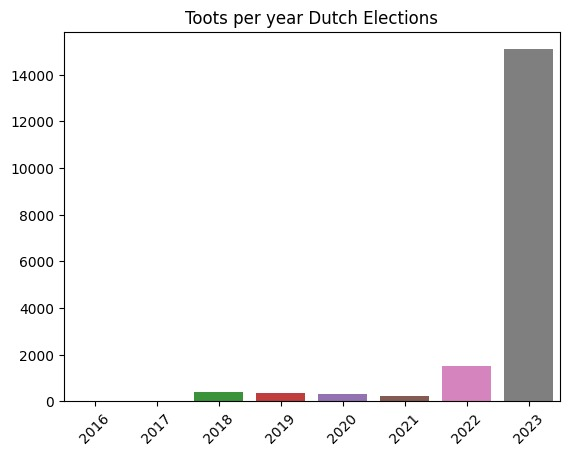
\includegraphics[width=3.25in]{media/dutch-elections-mastodon.jpeg}
  \caption{Bar chart of query word results, using general terms surrounding Dutch elections}
  \label{fig:electionstotal}
\end{figure}

\subsection{Activity of Political Parties (R1)}
With the list of terms extracted from the voting guide, the platform is queried for these terms and cross-referenced with party names, resulting in a dataset reflecting what parties get mentioned most topically on Mastodon.
The resulting graph in figure \ref{fig:partymentions} makes it clear that the Dutch socialist party (SP) is mentioned in conjunction with the topical terms the most.
The candlestick graph, where the wick represents the deviation of terms, shows that the SP also has the widest variety of topics mentioned.
One possible explanation is that their party initials are found in Dutch spelling quite commonly.
However, when isolation their initials, the results are the same, although this could still be the result of errors in our search endpoint syntax.
It is safe to assume the SP is an outlier, considering the second-highest activity party, is active on the platform itself and has a separate Mastodon instance

\begin{figure*}[ht]
  \centering
  \begin{subfigure}[h]{.49\linewidth}
    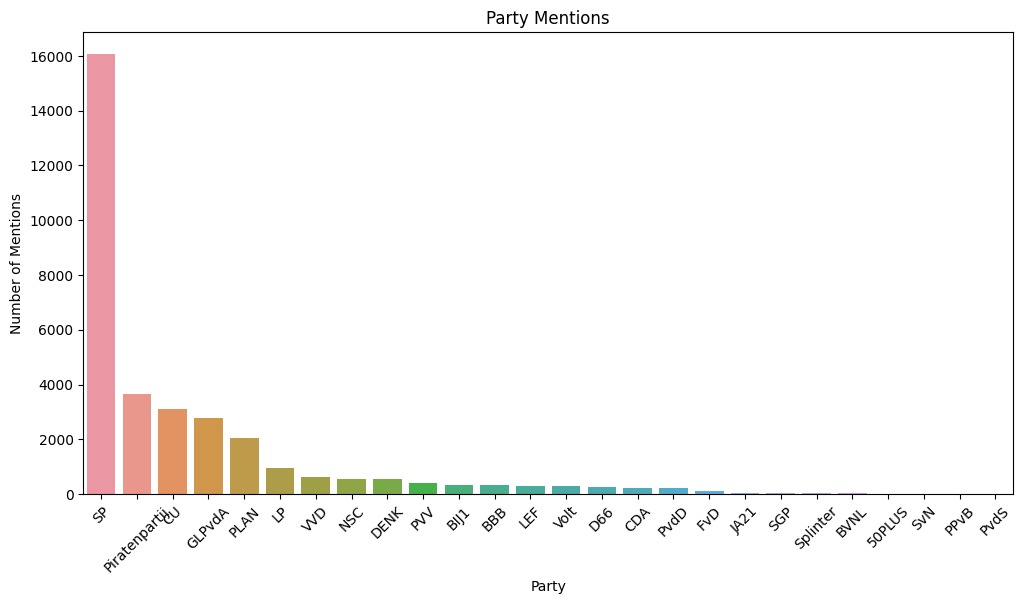
\includegraphics[width=\textwidth]{media/party-mentions.jpeg}
    \captionsetup{justification=centering}
    \caption{Bar chart showing individual political party mentions}
    \label{fig:partymentions}
  \end{subfigure}
  \begin{subfigure}[h]{.49\linewidth}
      \captionsetup{justification=centering}
      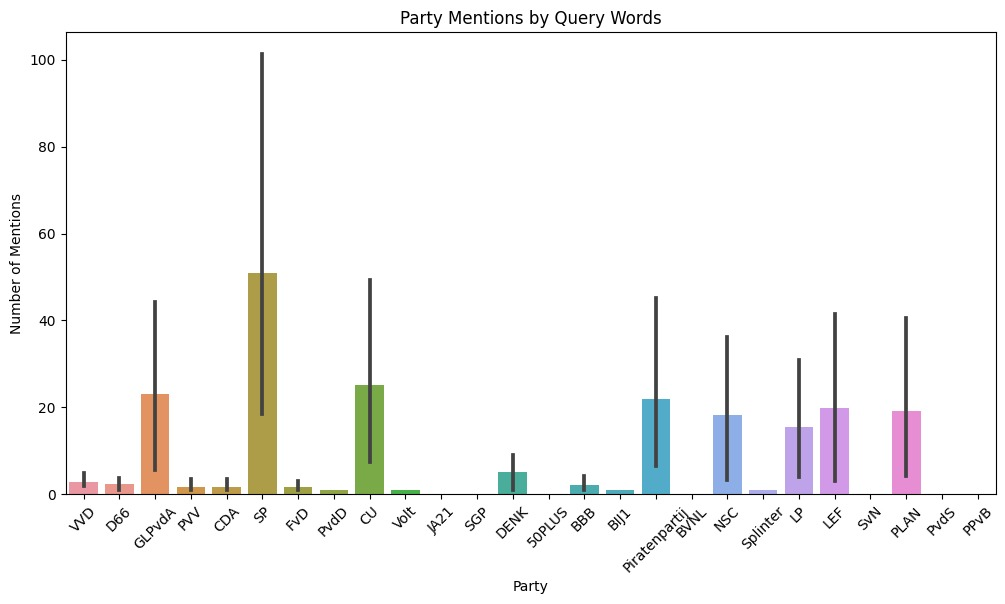
\includegraphics[width=\textwidth]{media/party-mentions-query-words.jpeg}
      \caption{Candlestick chart showing parties being mentioned based on topical query words. The wick represents the spread of unique topics}
      \label{fig:partycandle}
  \end{subfigure}
  \caption{Graphs visualizing party activity based on party name mentions and query words based on topics}
  \label{fig:results}
\end{figure*}

Activity around parties seems to focus on a small set of parties.
The second-highest mention, which seems like a more realistic activity hotspot, is the Piratenpartij.
Piratenpartij has its own Mastodon instance and multiple accounts, which also have the most activity itself, when compared to other party accounts on the platform, more of this is shown in the subsection for (R3).
Their deviation in figure \ref{fig:partycandle} also shows they are talked about in conjunction with a wide variety of topics.
Interestingly, the GL-PvdA party comes very close to the Piratenpartij, even though they are not active on the platform themselves.
An easy explanation would be, that this party has a lot of young voters and was mentioned in passing quite often because of their fusion (they used to be two separate parties).
Moreover, a large group of their constituents is known to be active in online discourse on other social media as well, as well as the sister party of the SP aimed at teenagers. 

\textbf{Finding M1:} \textit{Very few parties get mentioned, however, the parties that are mentioned are actively discussed. The cross-referencing might be influenced by the prevalence of the initials of parties in the Dutch language.}

\subsection{Election-related topics and query words (R2)}
The related topics mentioned per party mention show an interesting spread when plotted.
A hot topic, reasonably, is climate (and climate change) and “economy”, which in hindsight, might have been too general of a term, that etymologically contains most other terms as well.
These topics get mentioned almost exclusively by left-leaning parties, although it must be noted that almost all parties that have a reasonable amount of activity are left-leaning.
When comparing this chart to the activity around parties, it becomes clear certain queries result in actual political discourse toots and queries that don't have that much activity.
Most mentions group around the active parties, while other mentions are so sparse and distributed, that it seems more like the discourse is somewhat evenly spread across topics when the party and topic itself get mentioned by users.
There is no clear distinction in the actual difference of discourse between parties.
\begin{figure}[ht]
  \centering
  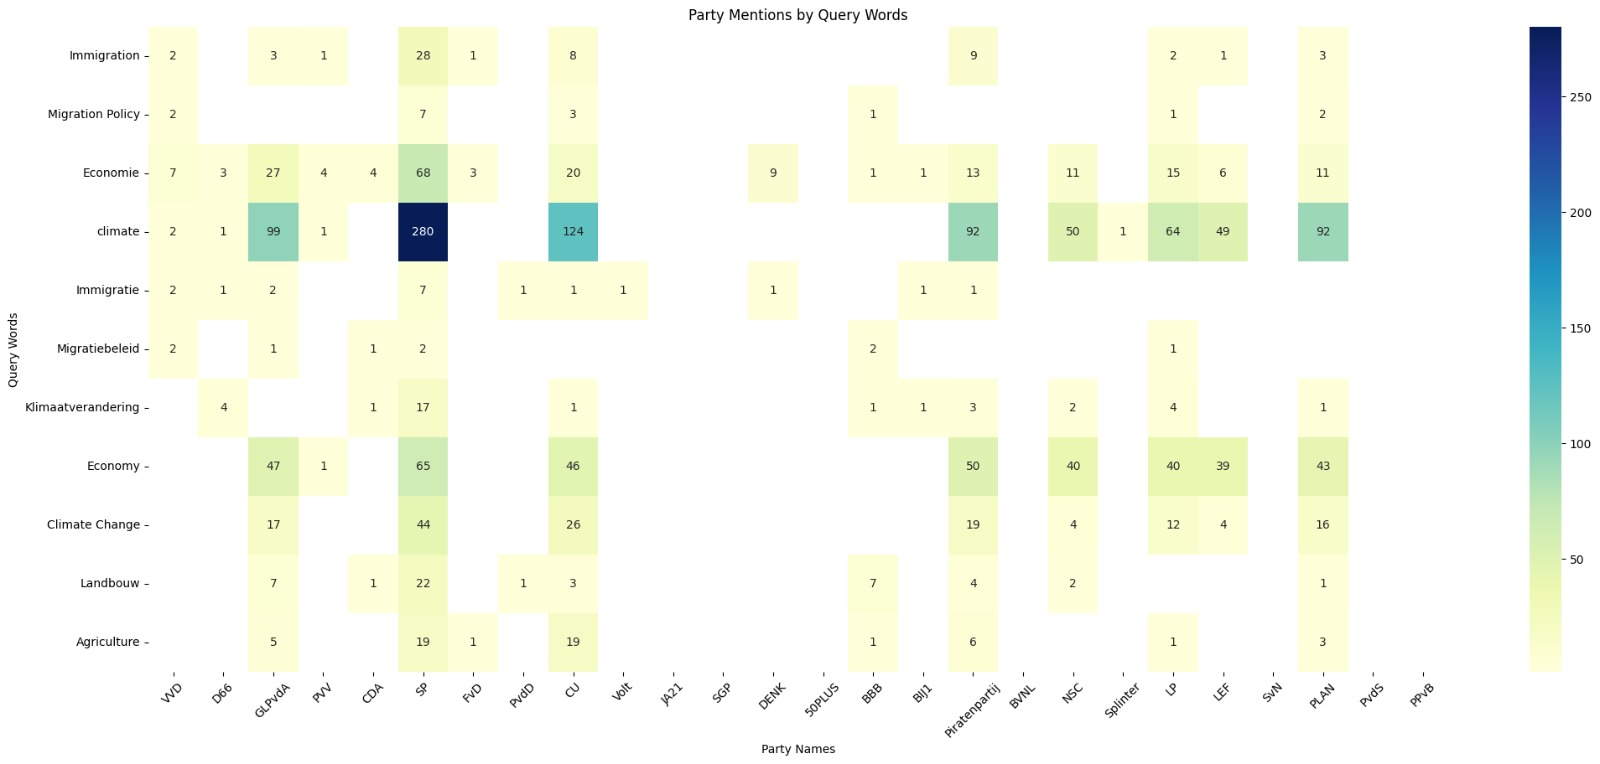
\includegraphics[width=\linewidth]{media/party-mentions-topics.jpeg}
  \caption{Party mentions related to topics}
  \label{fig:topic}
\end{figure}


\textbf{Finding M2:} \textit{Overall discourse seems to be on similar topics, only showing up in searches surrounding parties that have activity on the platform}

\subsection{Analysis of Party accounts and servers (R3)}
To more easily convey what parties have adopted the network, multiple queries have been performed, and analysed to find accounts connected to parties.
A list of all parties, including their nicknames and different spellings of abbreviations or those nicknames is looped through and queried in conjunction with different terms like “official”, “party”, “House of Representatives”, or “elections”, albeit in Dutch.
These queries resulted in the tree of different party accounts, as seen in figure \ref{fig:partynetwork}.

Noticeably, some parties are not active on the main server but instead have made their own server.
The Piratenpartij and Bij1 both have their own server, where the Piratenpartij server is quite active, at least compared to Bij1's server.
This also does not surprise from a political point of view, as the Piratenpartij, was founded to legislate internet laws and protect net neutrality.
The self-proclaimed radical left Bij1 party also occasionally mentions their need to operate in decentralized structures and hierarchies in their news and SNS outings.
The distinction between servers is more easily seen in figure \ref{fig:servernetwork} which branches to parties starting from the server as opposed to branching off from the party.

\begin{figure}[ht]
  \centering
  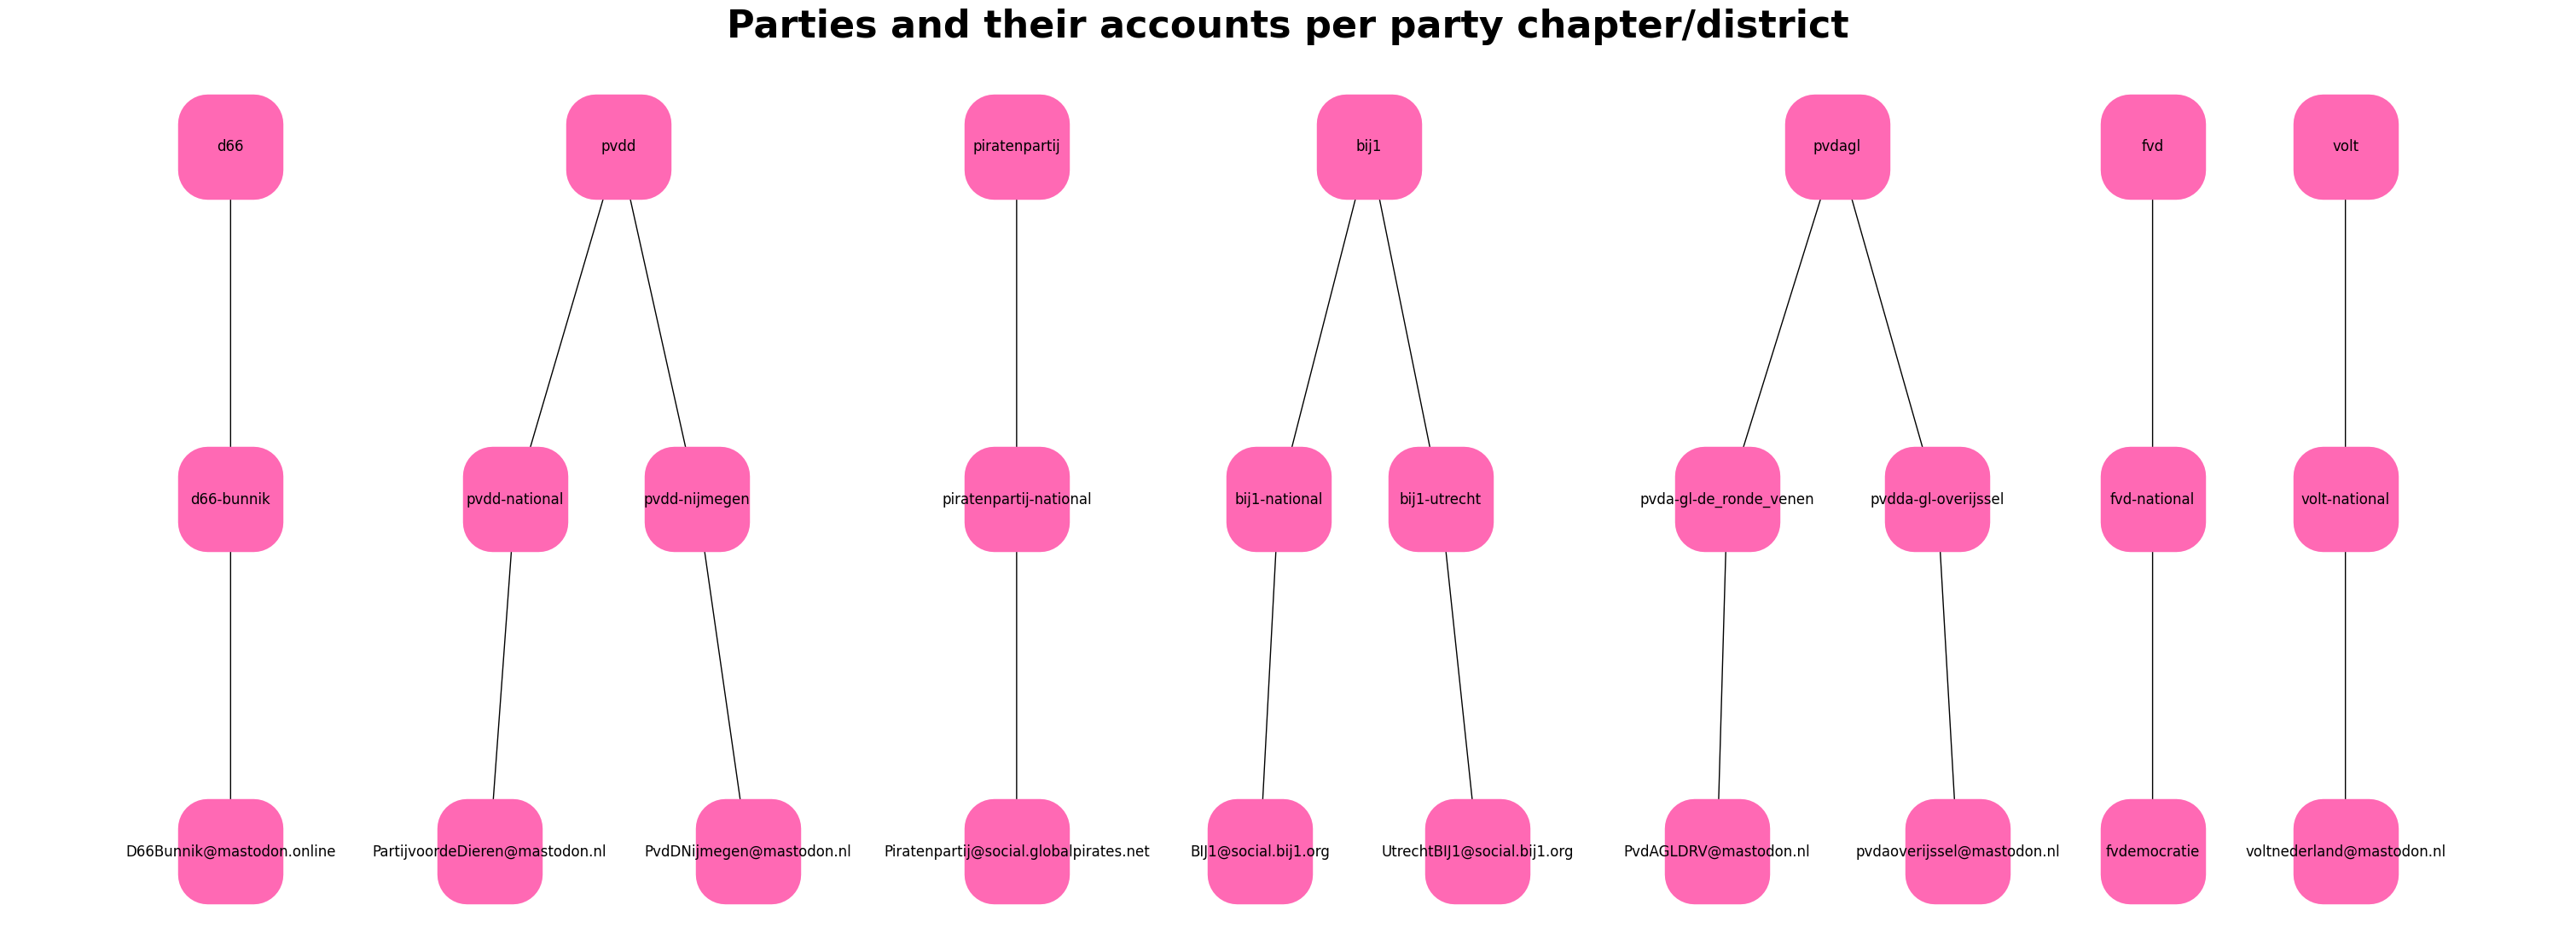
\includegraphics[width=\linewidth]{media/chapter.png}
  \caption{Tree of party accounts, branching from their district}
  \label{fig:partynetwork}
\end{figure}

\begin{figure}[ht]
  \centering
  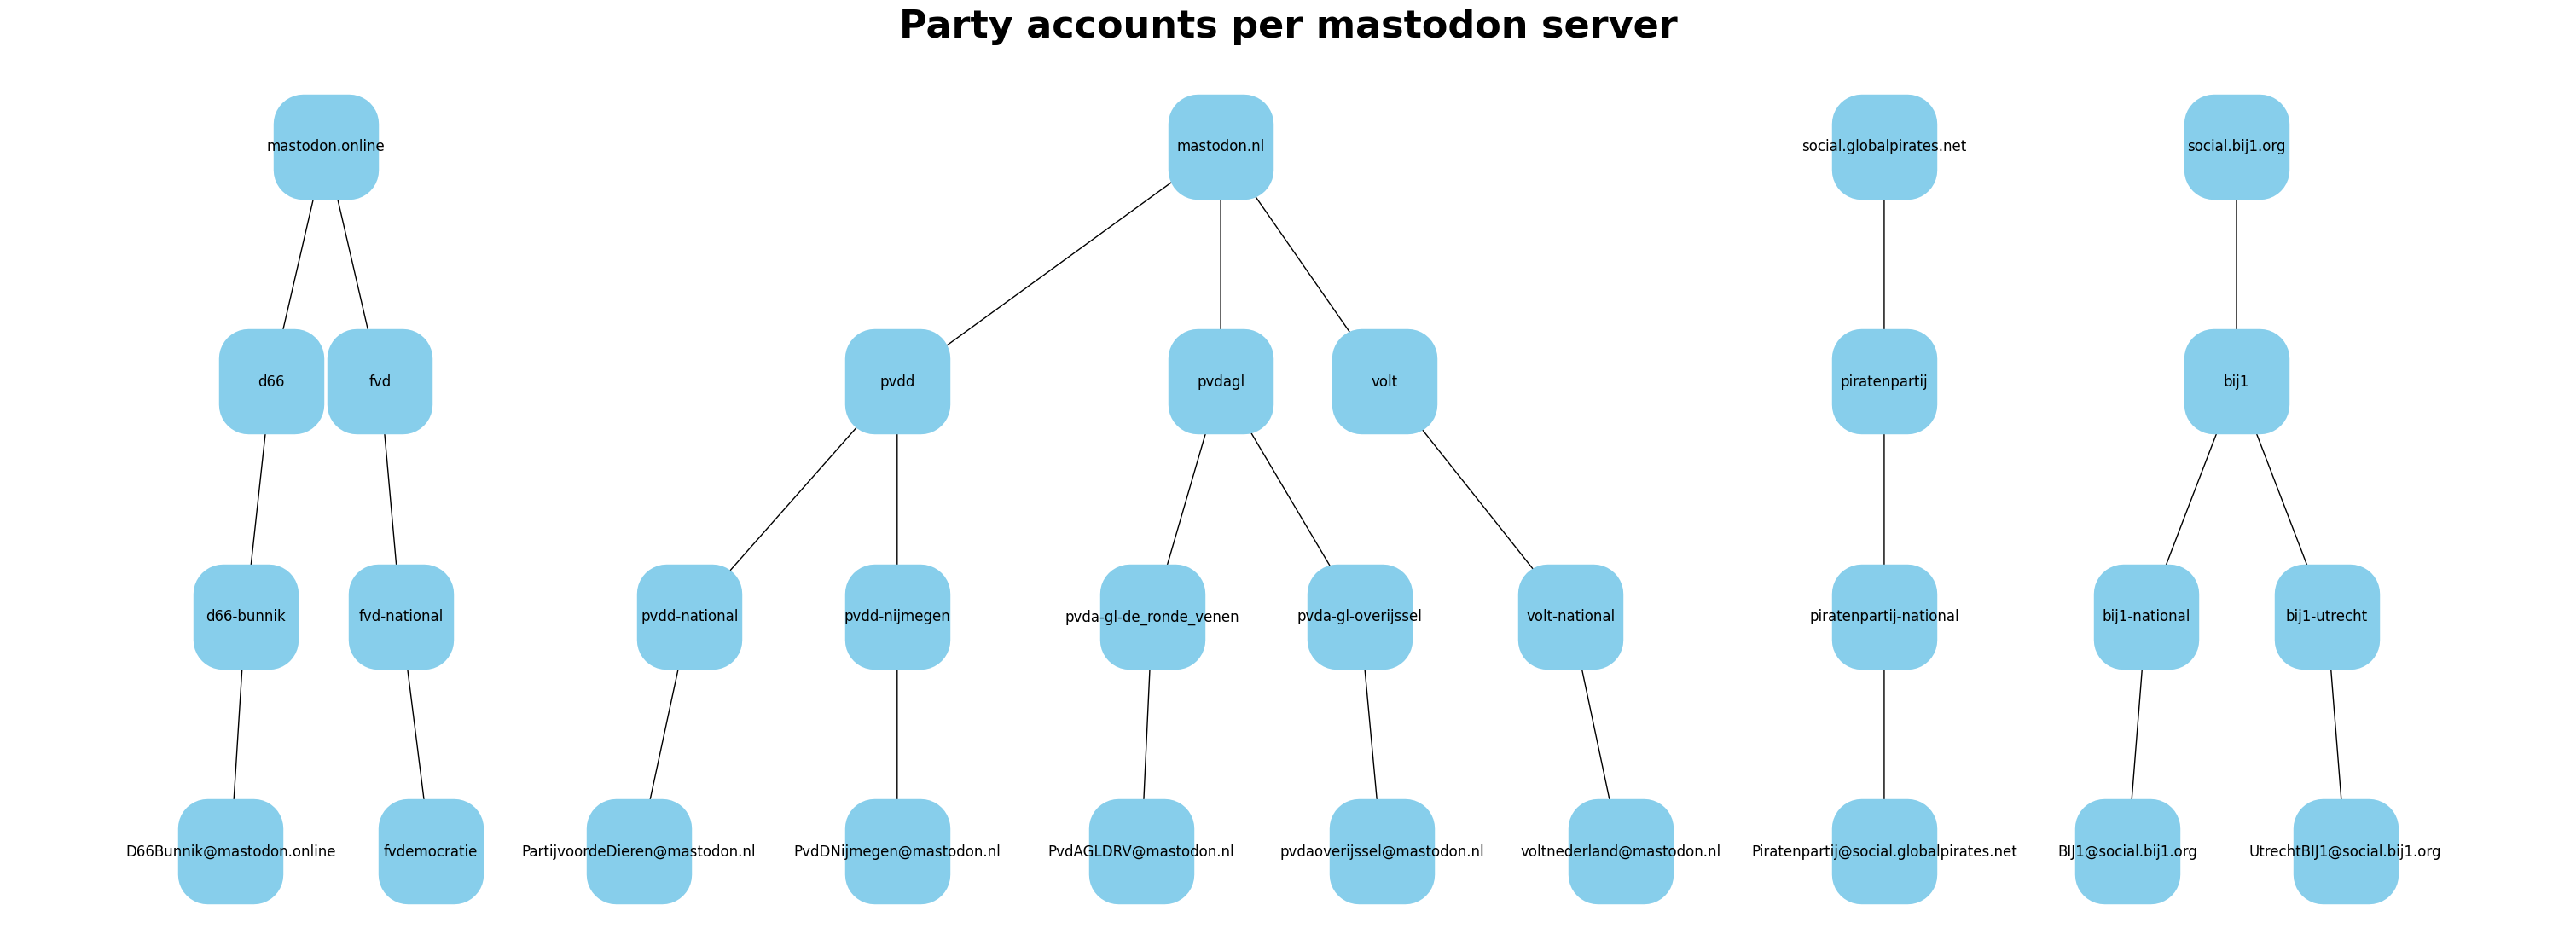
\includegraphics[width=\linewidth]{media/server.png}
  \caption{Tree of party accounts, branching from their respective server}
  \label{fig:servernetwork}
\end{figure}

\begin{figure*}[ht]
  \centering
  \begin{subfigure}[h]{.49\linewidth}
    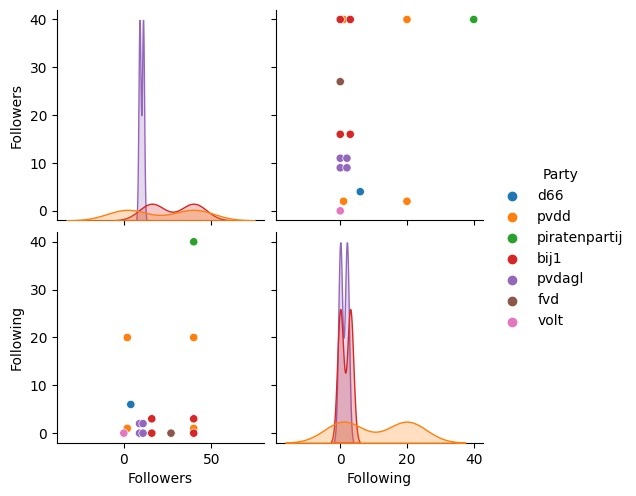
\includegraphics[width=\textwidth]{media/parties-following-counts.jpeg}
    \captionsetup{justification=centering}
    \caption{Party followers and following counts based on party name}
    \label{fig:partyfollowers}
  \end{subfigure}
  \begin{subfigure}[h]{.49\linewidth}
      \captionsetup{justification=centering}
      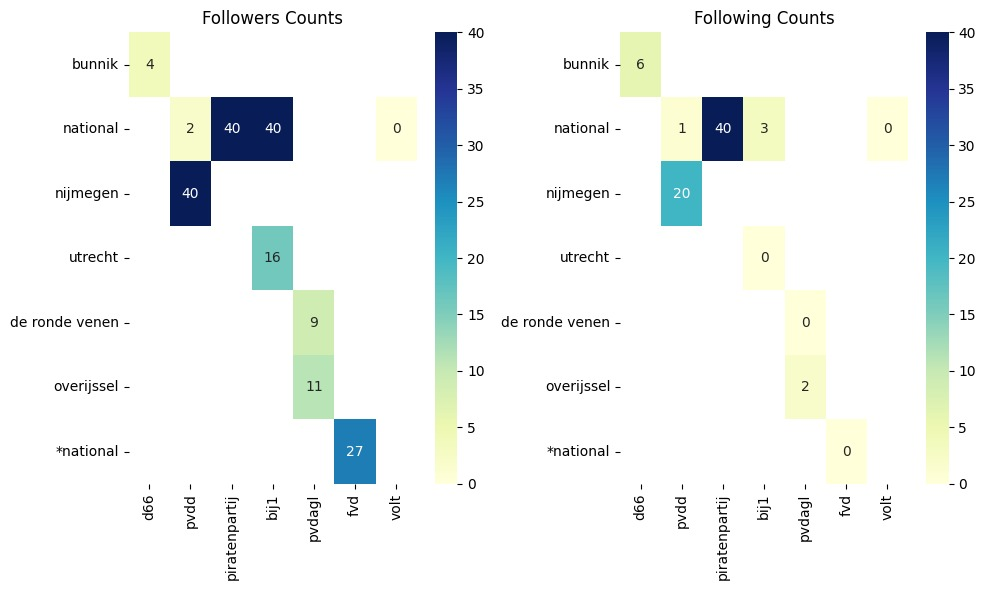
\includegraphics[width=\textwidth]{media/parties-following-region-counts.jpeg}
      \caption{Party followers and following counts based on sub instance and region}
      \label{fig:partyfollowingregions}
  \end{subfigure}
  \caption{Graphs visualizing parties and follower counts}
  \label{fig:partyfollowerstotal}
\end{figure*}


\textbf{Finding M3:} \textit{Out of all parties, 7 parties are present on Mastodon and 2 have their own instances.}
